% Topic 5 manuscript (English). Generated by paper/build.py from the registered runs;
% edit this template or sections/*.tex, never the generated manuscript.tex.
\documentclass[a4paper,preprint,12pt,authoryear]{elsarticle}
\usepackage{amsmath,amssymb}
\usepackage{booktabs}
\usepackage{graphicx}
\usepackage[table]{xcolor}
\usepackage[hidelinks,hypertexnames=false]{hyperref}
\usepackage[capitalise,noabbrev]{cleveref}
\usepackage{microtype}
\usepackage{float}
\setlength{\emergencystretch}{3em}
\pdfpagewidth=\paperwidth \pdfpageheight=\paperheight
\renewcommand{\appendixname}{Appendix}
\makeatletter
\g@addto@macro\appendix{\@addtoreset{table}{section}\@addtoreset{figure}{section}}
\makeatother
\journal{Comput. Educ.: Artif. Intell.}

\begin{document}
\begin{frontmatter}

\title{When failing tests are not enough: repair-grounded evaluation of misconception clustering for introductory C programs}

\begin{abstract}
Clustering failed submissions by the test cases they fail, and explaining clusters with IF--THEN rules, is a common proposal for telling instructors which misconceptions a large class shares, yet whether such clusters group programs by the mechanism of their errors is rarely tested for lack of labels. We build the labels without annotation. Replaying 8,607 C90 submissions of a public corpus in an isolated runner (98.42\% agreement with the historical grader), we reduce each failing program and the same student's next passing program to a verified minimal repair by delta debugging, and classify it into twelve program-level mechanisms; a second benchmark injects single mechanisms into accepted programs. Under a pre-registered protocol, identical test signatures mixed mechanisms: no function of the test-outcome representation could assign more than 73.9\% of 339 real and 50.7\% of 3,320 injected items correctly, and 81.6\% of injected pairs sharing a signature differed in mechanism. Label-free descriptors of how output deviates from the oracle raised this ceiling beyond a granularity-matched null and, on controlled data, raised the adjusted Rand index of K-means clusters from 0.09 to 0.33; on real repairs the gain (0.29 to 0.35) was not reliable, and the descriptors did not beat simpler output relations. A frozen code embedding clustered mutants by their source program rather than by mechanism. ILA-2 rules over problem-agnostic deviation attributes transferred to unseen assignments of the controlled benchmark (macro-F1 0.35). Output evidence, not larger models, is the cheapest route to mechanism-level feedback.

\end{abstract}

\begin{keyword}
programming education \sep misconceptions \sep clustering \sep program repair \sep rule induction \sep educational data mining
\end{keyword}

\end{frontmatter}

\section{Introduction}\label{sec:intro}

Instructors of large introductory programming courses cannot read every failed submission, yet they would like to know what the class as a whole gets wrong so that they can re-teach it. A popular answer is to cluster failed submissions and to summarise each cluster for the instructor. In the most common formulation, each submission is an object described by attribute--value pairs that record which test cases it fails (an object--attribute--value, OAV, representation), the objects are clustered with K-means or a Hamming-distance method, and production rules of the form IF~\emph{symptom} THEN~\emph{misconception} are induced to explain the clusters. The appeal is clear: test outcomes are available in every autograder, the representation is interpretable, and the rules read like teaching advice.

Whether such clusters group submissions by the \emph{mechanism} of the error is rarely tested, for a simple reason: public datasets of failed programs do not come with mechanism labels, and asking experts to label thousands of programs is expensive and hard to reproduce. Without labels, cluster quality is judged by internal indices such as silhouette, or by the fidelity of surrogate rules to the clusters. Neither says whether two programs that fail the same tests fail them for the same reason. Two programs can print the same wrong number because one loop stops one element early and another initialises an accumulator wrongly; conversely, one misunderstanding can make different tests fail depending on how the student wrote the rest of the program.

This paper builds the missing evaluation data without new annotation, and uses it to test the classic pipeline. Our starting point is that a student's own later submission often repairs the failed one. We replay a public corpus of 8,607 C90 submissions \citep{orvalho2024cpack} in an isolated runner, pair each failing submission with the same student's next passing submission, and use delta debugging to reduce their difference to a verified minimal repair, i.e., the smallest set of changed lines that, applied to the failing program, makes it pass every test. A deterministic classifier assigns this repair to one of twelve program-level categories, from loop boundaries to output format. The labels are therefore grounded in executed evidence rather than in judgement, and every one of them can be re-derived. Because real repairs are imbalanced and sometimes mix several changes, we add a second benchmark of controlled single-edit mutants of accepted programs whose category is known by construction.

With these two benchmarks we ask four questions. How much mechanism information do test-case signatures lose? Do label-free descriptions of \emph{how} the output deviates from the oracle recover mechanisms better at the same clustering budget? Do IF--THEN rules induced with the Inductive Learning Algorithm (ILA) and its noise-tolerant variant ILA-2 \citep{tolun1998ila,tolun1999ila2} generalise to new students and new assignments? And do frozen neural code embeddings cluster by mechanism or by author and program? All hypotheses, representations, weights and statistical rules were registered before the evaluation, and every departure is recorded as a dated amendment.

Our contributions are:
\begin{enumerate}
\item a reproducible, isolated replay of C-Pack-IPAs with an oracle audit against the historical grader (98.42\% agreement over 28,081 test verdicts) and a second independent replay (99.68\% agreement);
\item a repair-grounded benchmark of 750 verified minimal student repairs (339 single-mechanism labels) and a controlled benchmark of 3,320 single-edit mutants, sharing one taxonomy and one classifier;
\item execution-deviation OAV, a label-free and problem-agnostic representation of output deviations, and an evaluation protocol with an identifiability ceiling and a granularity-matched null;
\item pre-registered evidence that test signatures mix mechanisms (at most 73.9\% of real and 50.7\% of injected items are identifiable from them), that output-deviation evidence recovers mechanisms better on controlled data but not reliably on real repairs, that ILA-2 rules over it transfer to unseen assignments, and that a frozen code embedding clusters programs by origin.
\end{enumerate}
We release the replay runner, benchmarks, protocol and analysis code. Throughout, a label describes what changed in the program; it is not a claim about what the student believed.

\section{Related work}\label{sec:related}

\paragraph{Misconceptions and logic errors of novice programmers.}
Reviews of introductory programming describe misconceptions about variables, control flow, parameter passing and the notional machine that executes a program \citep{sorva2013notional,qian2017misconceptions}. Error studies distinguish slips from errors that follow from a wrong model of the language or task \citep{altadmri2015compilations,hermans2021brain}. \citet{ettles2018logic} classified logic errors of CS1 students into algorithmic errors, misinterpretations of the task and misconceptions, and found misconceptions to be the most frequent and the hardest to resolve. Misconception-driven feedback can help students when the misconception is known in advance \citep{gusukuma2018misconception}, and interactive instruments that ask students to predict program behaviour can elicit misconceptions directly \citep{lu2024smol}. These studies motivate automatic grouping of errors, but they also show that a program alone rarely reveals which belief produced it; we therefore evaluate program-level mechanisms and keep cognitive claims out of scope.

\paragraph{Clustering student programs.}
OverCode clusters correct solutions by normalised code \citep{glassman2015overcode}, and Clara clusters correct solutions by dynamic equivalence to repair incorrect ones \citep{gulwani2018clara}. For incorrect submissions, \citet{kaleeswaran2016semisupervised} cluster by repair strategy so that an instructor fixes one representative per cluster; MistakeBrowser clusters incorrect submissions by the code transformations that students applied when they fixed their own programs \citep{head2017mistakebrowser}; TraceDiff contrasts the traces of a buggy program and its closest fix \citep{suzuki2017tracediff}. Program embeddings learned from code and execution have been used to propagate feedback \citep{piech2015embeddings}, and \citet{shi2021misconception} clustered embeddings of incorrect block-based programs to help experts discover misconceptions. For C, InvAASTCluster combines dynamic invariants with abstracted syntax trees \citep{orvalho2025invaast}, and MENTOR couples clustering, formula-based fault localisation and LLM repair \citep{orvalho2026mentor}. These systems use repairs or correct solutions as part of the method. We use the student's own later repair only to construct evaluation labels, and ask how well representations that are available \emph{before} any repair recover them.

\paragraph{Mining misconceptions with learned models.}
Subtree-attention models localise logical errors from correctness labels alone \citep{hoq2025sann}, pattern-based knowledge components are extracted from student code with representation learning and clustering \citep{edm2026patternkc}, and LLMs discover misconceptions from sets of student code samples in McMining, whose benchmark injects known misconceptions into Python code \citep{alhossami2026mcmining}. Recent classroom tools cluster LLM-identified errors for instructors \citep{sigcse2026realtime}, ground tutoring in known misconceptions \citep{sigcse2026tutor}, or refine automatically detected signals with expert review \citep{aruleba2026ukicer}. PyMETA shows that diagnosis accuracy depends strongly on how the gold label is defined: prompted models that label the first execution error well agree far less with expert repair paths \citep{li2026pymeta}. Our study shares this concern and makes the label definition explicit, verifiable and reproducible.

\paragraph{Benchmarks, mutants and repairs.}
C-Pack-IPAs provides C90 submissions of 25 assignments with anonymised student identifiers, tests and historical grading logs \citep{orvalho2024cpack}; ITSP is an earlier benchmark of buggy and corrected C programs \citep{yi2017itsp}. Mutation analysis injects controlled faults; mutant detection correlates with real-fault detection in software testing \citep{just2014mutants}, and conceptual mutants built from students' wrong examples expose specification misconceptions \citep{prasad2024conceptual}. Delta debugging isolates a minimal failure-inducing difference between a failing and a passing configuration \citep{zeller2002ddmin}. We combine these ideas: we replay the corpus, reduce each student's own repair to a verified minimal change, and pair these labels with controlled single-mechanism mutants.

\paragraph{Rule induction.}
The Inductive Learning Algorithm (ILA) extracts production rules class by class from attribute--value examples \citep{tolun1998ila}; ILA-2 adds a penalty factor that tolerates noisy data \citep{tolun1999ila2}. ILA is sometimes listed alongside clustering methods, but it is supervised rule induction, and we use it as such: to state IF--THEN rules that map execution evidence to mechanisms and to measure how well such rules hold on students not used to induce them.

\section{Data and benchmark construction}\label{sec:data}

\subsection{Corpus and isolated replay}\label{sec:replay}
We use the canonical submissions of C-Pack-IPAs release~26 \citep{orvalho2024cpack}: 8,607 C90 programs by 246 anonymised students for 25 assignments of three laboratory classes, with 106 input/output tests. The historical logs record a verdict per test but often no output for passing tests, and 9,425 test cells were never executed or not logged. To obtain complete execution evidence we replayed every non-empty program in a research-only container: no network, read-only root file system, all Linux capabilities dropped except those needed to switch to an unprivileged per-run user, and resource limits of 3~s CPU, 5~s wall time and 512~MiB of address space per test. Programs were compiled with \texttt{gcc} 12.2.0 and the course flags (\texttt{-ansi -pedantic -Wall -Wextra}); because the course also used \texttt{-Werror}, we recorded whether compilation was warning-free instead of rejecting the program. The container returns raw output bytes; oracles stay on the host, which decides every verdict.

The replay agreed with 98.42\% of the 28,081 historical test verdicts under the exact-match, zero-exit policy (selected on the training partition among four comparison policies; \cref{tab:audit}), reproduced the logged output of 96.1\% of historically wrong answers byte for byte, and matched the historical compilation outcome under \texttt{-Werror} semantics for 99.76\% of programs. A second, independent replay from a clean commit agreed on 99.68\% of test cells; the 56 programs whose outcomes differed between the two replays (likely undefined behaviour) were excluded from all items (amendment~A5).

\begin{table}[t]
\centering
\caption{Agreement (\%) of the isolated replay with the historical per-test verdicts under four output comparison policies. The policy was chosen on the training partition before any mechanism label existed.}\label{tab:audit}
\small
\begin{tabular}{lrrr}
\toprule
Comparison policy & Train & Validation & Test \\
\midrule
Exact output, exit status 0 (selected) & 98.23 & 99.04 & 98.52 \\
Exact output, any exit status & 98.16 & 98.70 & 98.36 \\
Ignore trailing whitespace & 89.03 & 89.75 & 91.13 \\
Whitespace-separated tokens & 83.88 & 86.22 & 86.47 \\
\bottomrule
\end{tabular}
\end{table}

\subsection{Split}
Submissions were split before any label existed into training, validation and test partitions (70/15/15\% of connected components) such that all submissions of a student, across years and assignments, and all byte-identical sources fall into one partition. Every derived item inherits the partition of the submission it comes from.

\subsection{Repair-grounded labels}\label{sec:real}
For every failing submission (at least one test not passed) we looked for the same student's next submission to the same assignment in the same year that passed every test. For each such repair event we kept the latest failing attempt before it (amendment~A2), giving 750 failing--repaired pairs. The line difference between the two programs, ignoring indentation, was split into hunks. Hunk-level delta debugging \citep{zeller2002ddmin} then searched for a 1-minimal subset of hunks whose application to the failing program makes it pass every test, executing every candidate in the isolated runner (budget 64 probes per pair). Both endpoints were re-verified in the same runner before the search. The verified minimal change was classified into one of twelve program-level categories (\cref{tab:taxonomy}) by a deterministic classifier that works on each verified line hunk: whole statements that were inserted or deleted are recognised after sliding the token run to statement boundaries, identical lines that were deleted and re-inserted elsewhere are placement changes, and every other changed token is attributed to its innermost role-defining syntactic context (loop header, branch condition, initialiser, output format, and so on). A pair receives a single-mechanism label only when its minimal repair falls into exactly one category other than \textsc{Other}; repairs spanning several categories are kept as \textsc{Multi} and excluded from the primary gold. The repairing submission, the patch and the label are never used as features.

\subsection{Controlled mechanism injection}\label{sec:injected}
Real repairs are ecologically valid but noisy, imbalanced and specific to what students happened to do. We therefore also built a controlled benchmark. From accepted, warning-free programs (at most 40 per assignment, one per student and year) we generated single-edit mutants with operators aligned with the same taxonomy: strictness of a loop or branch comparison, logical connective, loop start, constant initialiser, arithmetic operator, removed float cast or float literal, printf precision, dropped trailing newline, letter case of output text, deleted statement, duplicated statement, and statements moved into a loop. One random site per category and source was mutated with a fixed seed. A mutant was kept only if it compiled without warnings and failed at least one test, i.e., if it could have been a real failing submission of the course. A unit test checks that the classifier of \cref{sec:real} assigns every operator's inverse edit to the operator's category, so both label sets share one definition.

\begin{table}[t]
\centering
\caption{Program-level mechanism taxonomy. A category describes what the verified minimal repair (or the injected edit) changes; the right column lists misconception hypotheses an instructor may check, not diagnoses.}\label{tab:taxonomy}
\small
\begin{tabular}{p{2.9cm}p{4.9cm}p{4.6cm}}
\toprule
Category & The minimal change edits\dots & Hypotheses to check \\
\midrule
Loop boundary & condition, start or update of a loop & off-by-one, 0- vs 1-based ranges \\
Branch condition & condition or structure of if/switch/else & boundary of comparisons, \texttt{\&\&} vs \texttt{||} \\
Initialisation & a declaration initialiser or constant assignment outside loops & accumulator or extremum initialisation \\
Computation & operators or operands of assignments, returns, printed expressions & formula, precedence \\
Numeric type & types, casts, float literals, math functions & integer division \\
Output format & printf conversion specifications & precision, width \\
Output text & literal output text or print-only statements & reading the output specification \\
Input & scanf/getchar calls & input format, end of file \\
Statement placement & a moved statement or brace & scope of blocks, reset inside loops \\
Missing statement & inserted whole statements & missing update or case \\
Extra statement & deleted whole statements & duplicated update, debug output \\
Control flow & break/continue/return & premature exit \\
\bottomrule
\end{tabular}
\end{table}

\section{Methods}\label{sec:methods}

\subsection{Object--attribute--value representations}\label{sec:reps}
Every failing program (the object) is described by categorical attributes. All representations are computed from the failing program and its own replayed runs only. Vocabularies are fitted, without labels, on training-partition failing submissions of the same assignment; values unseen in training are mapped to \emph{unknown}.
\begin{itemize}
\item \textbf{Outcomes} (the test-case OAV of the classic formulation): one attribute per test with value pass, fail, runtime error or timeout.
\item \textbf{Structural}: presence of 16 C constructs (loop kinds, inclusive/strict comparisons, subscripts, pointers, \dots).
\item \textbf{Outcomes+stdout} and \textbf{Combined+stdout}: the strongest representations of our earlier pipeline, adding per-test output relations (exact, whitespace, empty, another test's oracle, different) and edit-distance bands, and in the combined case also the structural block.
\item \textbf{Deviation} (proposed): the outcome block plus, per test, nine label-free descriptors of \emph{how} the output deviates from the oracle---line count, trailing newline, whitespace-only difference, relation between corresponding numbers (off by one, truncated, precision, sign, zero, scale, format only), relation between words (case only, typo, missing or extra words), position of the first differing line, prefix relations and equality with another test's oracle---and the same descriptors aggregated over failing tests, which are problem-agnostic.
\item \textbf{Evidence} (proposed): deviation plus eighteen static code cues (strict and inclusive loop comparisons, non-zero loop start, constant initialisers, division without a float operand, casts, printf precisions, output inside loops, output words absent from every oracle, \dots).
\item \textbf{Embedding}: a frozen code embedding of the raw source (Qwen3-Embedding-0.6B, \citealt{zhang2025qwen3embedding}), L2-normalised.
\end{itemize}
Block masses were fixed in the registered protocol before any evaluation and were not tuned (outcomes $1$; outcomes+stdout $0.6/0.4$; combined+stdout $0.48/0.12/0.4$; deviation $0.3$ tests, $0.4$ per-test deviation, $0.3$ aggregate; evidence $0.2/0.3/0.2$ and $0.3$ code cues).

\subsection{Clustering and rules}
Each assignment's failing programs form a cohort that is clustered transductively. K-means runs on the one-hot encoding scaled by the square root of the attribute weights (seeds 7, 42, 91), and agglomerative clustering uses average linkage on the weighted Hamming distance; embeddings use Euclidean K-means and cosine distance. The primary analysis gives every method the number of gold categories present in the cohort (\emph{oracle} $k$, capped by the number of distinct representation patterns), which isolates the representation from model selection; a secondary analysis selects $k\in[2,10]$ by silhouette without labels. The cheapest baseline groups identical test signatures.

For IF--THEN rules we use ILA \citep{tolun1998ila} and ILA-2 \citep{tolun1999ila2} over problem-agnostic attributes: the aggregated deviation descriptors and code cues (\emph{evidence}), or only the aggregated outcome state and the fraction of failing tests (\emph{outcome summary}). Rules are induced from training-partition labels, applied in precision order, and examples matched by no rule are counted as abstentions and errors. The ILA-2 penalty factor was the only quantity tuned, on the validation partition among $\{1,2,5\}$. We compare with a depth-4 CART tree on the same attributes and with the majority class, on seen assignments with unseen students, and on unseen assignments (laboratory~4) with unseen students.

\subsection{Measures and registered hypotheses}\label{sec:hyp}
The primary measure is the adjusted Rand index (ARI; \citealt{hubert1985ari}) between a cohort's clusters and its gold categories, macro-averaged over cohorts with at least six items and two categories; we also report adjusted mutual information \citep{vinh2010ami}, pairwise F1 and purity. The \emph{identifiability ceiling} of a representation is $\sum_b \max_y n_{b,y}/N$ over its buckets $b$ of identical attribute vectors: no clustering or classifier that only reads the representation can exceed it. Because deviation OAV refines the outcome OAV, its ceiling cannot be lower; we therefore compare it with the expected ceiling of a random refinement that splits every outcome bucket into sub-buckets of the same sizes (200 permutations).

The protocol, registered before any mechanism evaluation, states five hypotheses with falsification criteria (seven dated amendments were recorded before the sealed test run, six of them before any evaluation result; \cref{app:protocol}):
H1a, identical test signatures mix mechanisms (the upper 95\% bound of the mean outcome ceiling is below $0.95$);
H1b, the refinement added by deviation OAV carries mechanism information beyond its granularity;
H2, deviation OAV yields higher ARI than outcome OAV;
H3, evidence OAV yields higher ARI than the strongest earlier baseline, combined+stdout;
H4, ILA-2 rules over agnostic evidence reach a higher test macro-F1 than rules over the outcome summary on the real benchmark;
H5, on the injected benchmark, frozen code-embedding clusters align more with the source program than with the injected mechanism.
Differences are summarised by their mean over cohorts with a 95\% bootstrap interval (10{,}000 resamples) and Wilcoxon signed-rank tests with Holm correction; rule comparisons use a bootstrap over students. A hypothesis is supported only when the interval of the difference excludes zero in the stated direction on every benchmark it names. Because real single-mechanism items are sparse in the sealed test partition (0 eligible cohorts), the registered amendment A3 evaluates clustering on the real benchmark over full per-assignment cohorts (clustering fits nothing on labels); the injected benchmark is evaluated on test-partition cohorts, with full cohorts reported in the released results. Rule induction always trains on the training partition and is scored on the test partition.

\section{Results}\label{sec:results}

\subsection{Benchmarks}
Of the 750 repair events, 746 passed the endpoint checks and 743 reached a 1-minimal repair within the probe budget; 72\% of minimal repairs changed one or two line hunks. 54.4\% of the minimal repairs spanned more than one category and were excluded from the gold; the remaining 339 single-mechanism items are dominated by output text (the course graded output byte for byte), followed by computation, missing statements, branch conditions, loop boundaries, output format and control flow (7 of the 8 audited control-flow repairs added the \texttt{return 0} that C90 needs for a zero exit status). The controlled benchmark contains 3,320 mutants over nine categories; 16.6\% of candidate mutants passed every test and were discarded as equivalent on the suite. Full counts are released with the benchmark (\texttt{stats.json}).

\subsection{Test signatures mix mechanisms (H1a, H1b)}
Identical test signatures often hide different mechanisms (\cref{fig:ceiling}). The best any function of the test-outcome OAV can do is to assign 73.9\% of real items (mean ceiling 0.74, 95\% CI [0.70, 0.78]) and 50.7\% of injected items ([0.43, 0.59]) to their mechanism, so H1a is supported on both benchmarks. Put differently, 35.5\% of the 2,087 real pairs that share a test signature within an assignment have different mechanisms, and 81.6\% of the 2,901 injected pairs do. The refinement added by deviation OAV raises the ceiling by 0.080 [0.052, 0.112] on real and 0.172 [0.121, 0.224] on injected cohorts beyond a random refinement of the same granularity (H1b supported; Holm $p=0.0018$ and 0.0000). The extra distinctions therefore carry mechanism information rather than mere resolution.

\begin{figure}[t]
\centering
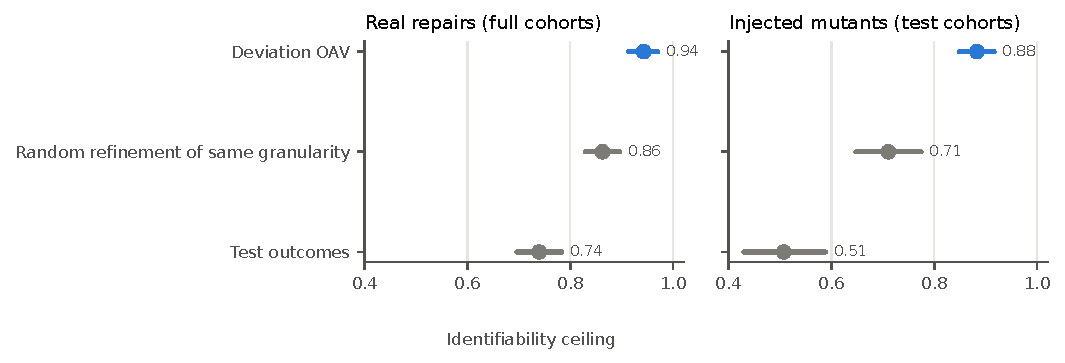
\includegraphics[width=\textwidth]{figures/ceiling_en.pdf}
\caption{Identifiability ceiling: the highest share of items that any function of a representation can assign to their mechanism. Deviation OAV exceeds both the test-outcome OAV and a random refinement with the same bucket sizes. Points are means over cohorts; bars are 95\% bootstrap intervals.}\label{fig:ceiling}
\end{figure}

\subsection{Clustering by mechanism (H2, H3)}
\Cref{tab:ari,fig:ari} report mechanism recovery at the same clustering budget. On the controlled benchmark, clusters of the test-outcome OAV barely agree with mechanisms (ARI 0.09, exact signatures 0.10), while deviation OAV reaches 0.33: a difference of 0.235 [0.143, 0.331] with K-means and 0.214 [0.117, 0.314] with HAC, larger in 16/20 cohorts. On real repairs the test-outcome OAV already reaches 0.29 because the dominant output-text category produces distinctive signatures; deviation OAV reaches 0.35 with K-means and 0.38 with HAC, but the differences (0.054, CI [$-$0.081, 0.182]; 0.086, CI [$-$0.025, 0.200]) are not reliable. H2 is therefore supported on the controlled benchmark only and, by the registered rule, not supported overall.

H3 is not supported: evidence OAV and the earlier combined+stdout baseline are indistinguishable on both benchmarks (differences $-$0.006 and 0.002). Simple output relations already capture most of what distance-based clustering can exploit; outcomes+stdout reaches 0.36 and 0.34. Selecting $k$ by silhouette instead of the oracle lowers all scores slightly and preserves the ordering (\cref{tab:ari}).

\begin{table}[t]
\centering
\caption{Mechanism recovery on the two benchmarks: mean ARI over cohorts (oracle $k$ unless stated) and mean identifiability ceiling. Real repairs: full per-assignment cohorts (amendment A3); injected mutants: sealed test-partition cohorts.}\label{tab:ari}
\small
\begin{tabular}{lrrrr}
\toprule
Representation & K-means & HAC & K-means, silh.\ $k$ & Ceiling \\
\midrule
\multicolumn{5}{l}{\emph{Real repairs}} \\
Test outcomes (classic OAV) & 0.292 & 0.292 & 0.239 & 0.739 \\
Outcomes + stdout & 0.363 & 0.367 & 0.313 & 0.907 \\
Combined + stdout & 0.306 & 0.334 & 0.314 & 0.980 \\
AST presence & 0.064 & 0.029 & 0.080 & 0.772 \\
Code cues & 0.141 & 0.157 & 0.105 & 0.931 \\
Code embedding & 0.060 & 0.077 & 0.063 & -- \\
Deviation OAV (ours) & 0.345 & 0.378 & 0.295 & 0.943 \\
Evidence OAV (ours) & 0.300 & 0.324 & 0.279 & 0.986 \\
Exact test signature & 0.281 & -- & -- & -- \\
\midrule
\multicolumn{5}{l}{\emph{Injected mutants}} \\
Test outcomes (classic OAV) & 0.093 & 0.084 & 0.088 & 0.507 \\
Outcomes + stdout & 0.338 & 0.299 & 0.332 & 0.839 \\
Combined + stdout & 0.335 & 0.293 & 0.309 & 0.914 \\
AST presence & $-$0.066 & $-$0.068 & $-$0.052 & 0.353 \\
Code cues & 0.009 & $-$0.009 & $-$0.020 & 0.654 \\
Code embedding & $-$0.115 & $-$0.104 & $-$0.114 & -- \\
Deviation OAV (ours) & 0.328 & 0.297 & 0.328 & 0.883 \\
Evidence OAV (ours) & 0.337 & 0.283 & 0.227 & 0.964 \\
Exact test signature & 0.096 & -- & -- & -- \\
\bottomrule
\end{tabular}
\end{table}

\begin{table}[t]
\centering
\caption{Registered hypotheses: mean difference over cohorts, 95\% bootstrap interval and verdict (H1a reports the mean outcome ceiling itself).}\label{tab:hyp}
\small
\resizebox{\textwidth}{!}{%
\begin{tabular}{lrllrll}
\toprule
 & \multicolumn{3}{c}{Real repairs} & \multicolumn{3}{c}{Injected mutants} \\
\cmidrule(lr){2-4}\cmidrule(lr){5-7}
Hypothesis & Mean & 95\% CI & Verdict & Mean & 95\% CI & Verdict \\
\midrule
H1a & 0.739 & [0.696, 0.783] & supported & 0.507 & [0.429, 0.588] & supported \\
H1b & 0.080 & [0.052, 0.112] & supported & 0.172 & [0.121, 0.224] & supported \\
H2 kmeans & 0.054 & [$-$0.081, 0.182] & not supported & 0.235 & [0.143, 0.331] & supported \\
H2 hac & 0.086 & [$-$0.025, 0.200] & not supported & 0.214 & [0.117, 0.314] & supported \\
H3 kmeans & $-$0.006 & [$-$0.097, 0.117] & not supported & 0.002 & [$-$0.055, 0.067] & not supported \\
H3 hac & $-$0.010 & [$-$0.111, 0.119] & not supported & $-$0.010 & [$-$0.060, 0.041] & not supported \\
H5 & -- & -- & -- & 0.834 & [0.695, 0.958] & supported \\
\bottomrule
\end{tabular}}
\end{table}

\begin{table}[t]
\centering
\caption{IF--THEN rules predicting the mechanism of test-partition students from problem-agnostic attributes, real repairs. Abstentions count as errors in macro-F1; selective accuracy is measured on answered items.}\label{tab:rules}
\small
\resizebox{\textwidth}{!}{%
\begin{tabular}{llrrr}
\toprule
Track & Model (attributes) & Macro-F1 & Coverage & Selective acc. \\
\midrule
Seen assignments & ILA (evidence) & 0.254 & 0.586 & 0.765 \\
Seen assignments & ILA-2 (evidence) & 0.256 & 0.690 & 0.700 \\
Seen assignments & CART (evidence) & 0.244 & 1.000 & 0.621 \\
Seen assignments & ILA (outcome summary) & 0.000 & 0.000 & 0.000 \\
Seen assignments & ILA-2 (outcome summary) & 0.130 & 0.828 & 0.583 \\
Seen assignments & CART (outcome summary) & 0.251 & 1.000 & 0.586 \\
Seen assignments & Majority class & 0.109 & 1.000 & 0.483 \\
Unseen assignments & ILA (evidence) & 0.354 & 1.000 & 0.500 \\
Unseen assignments & ILA-2 (evidence) & 0.354 & 1.000 & 0.500 \\
Unseen assignments & CART (evidence) & 0.381 & 1.000 & 0.500 \\
Unseen assignments & ILA (outcome summary) & 0.000 & 0.000 & 0.000 \\
Unseen assignments & ILA-2 (outcome summary) & 0.214 & 0.750 & 0.500 \\
Unseen assignments & CART (outcome summary) & 0.214 & 1.000 & 0.375 \\
Unseen assignments & Majority class & 0.136 & 1.000 & 0.375 \\
\bottomrule
\end{tabular}}
\end{table}

\begin{figure}[t]
\centering
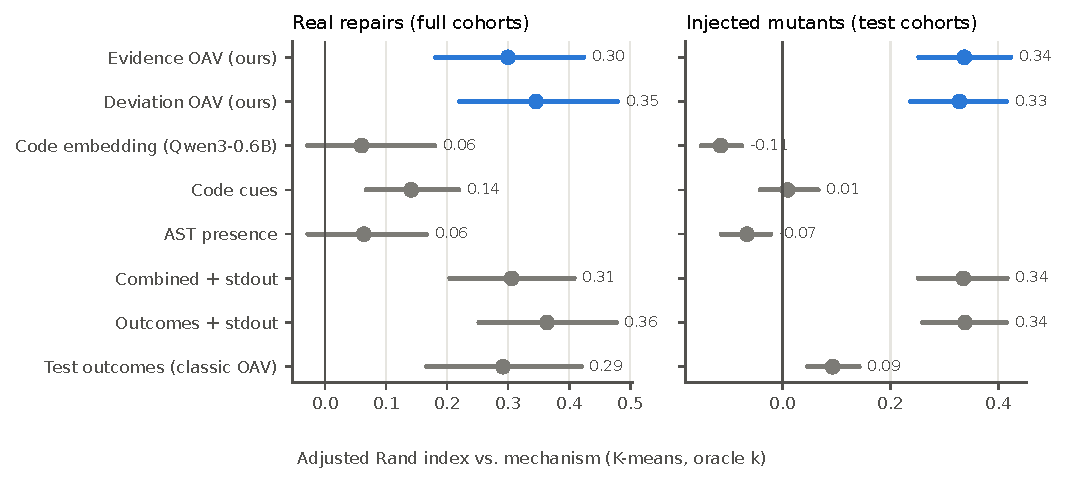
\includegraphics[width=\textwidth]{figures/ari_en.pdf}
\caption{Adjusted Rand index between clusters and mechanisms (K-means, oracle $k$). Blue: proposed representations; grey: baselines. Points are means over cohorts; bars are 95\% bootstrap intervals over cohorts.}\label{fig:ari}
\end{figure}

\subsection{Frozen code embeddings cluster programs, not mechanisms (H5)}
Qwen3-Embedding clusters of injected mutants agree more with the accepted program the mutant came from than with the injected mechanism, by 0.834 ARI (95\% CI [0.695, 0.958]; H5 supported). Their mechanism ARI is $-$0.11 on injected and 0.06 on real cohorts. Single-token changes that decide a program's behaviour barely move a general-purpose embedding, whereas authorship and solution style dominate it.

\subsection{IF--THEN rules (H4)}
ILA-2 rules over problem-agnostic evidence attributes predicted the mechanism of real test-partition items with macro-F1 0.26 (coverage 0.69, accuracy on answered items 0.70), against 0.13 for rules over the outcome summary and 0.11 for the majority class (\cref{tab:rules}). The difference, 0.094 [$-$0.011, 0.171], rests on the 29 single-mechanism items of the sealed test students and includes zero, so H4 is not supported. On the injected benchmark, where every category is represented, evidence rules reached macro-F1 0.65 on seen and 0.35 on unseen assignments, whereas outcome-summary rules reached 0.03 and 0.04. The noise-tolerant penalty of ILA-2 traded a little precision for much coverage: the original ILA answered 0.34 of injected test items with accuracy 0.94, ILA-2 answered 0.81 with accuracy 0.74. \Cref{tab:toprules} lists the highest-precision rules learned from real repairs; they read like the production rules of the classic formulation, but their conclusions are program-level mechanisms and their precision was measured on students not used to induce them.

\begin{table}[t]
\centering
\caption{The most precise ILA-2 rules induced from real training repairs (support: correct/matched training items).}\label{tab:toprules}
\small
\begin{tabular}{p{7.6cm}p{3.0cm}r}
\toprule
IF & THEN mechanism & Support \\
\midrule
the program has no output call & missing statement & 10/10 \\
the program has no input call & missing statement & 8/8 \\
printed numbers equal the oracle's but are written differently & output format & 8/8 \\
the trailing newline is as expected and fewer numbers than the oracle are printed & output text & 7/7 \\
the failing tests time out & loop boundary & 4/4 \\
the output is a truncated prefix of the oracle & output text & 78/79 \\
the output differs from the oracle only in whitespace & output text & 97/107 \\
the output contains words the oracle lacks & output text & 20/24 \\
\bottomrule
\end{tabular}
\end{table}

\subsection{Which mechanisms benefit (exploratory)}
Per category (\cref{app:categories}), test signatures recover output text (0.98), loop boundaries (0.88) and control flow (0.83) on real repairs, but not output format (0.00), branch conditions (0.24) or missing statements (0.37); with deviation OAV these rise to 0.69, 0.59 and 0.56. Averaged over categories, recovery rises from 0.54 to 0.71 on real and from 0.50 to 0.72 on injected cohorts. The gains of output evidence thus concentrate in the minority mechanisms that a cohort-level ARI weighs little, which explains why the real-benchmark ARI difference is small.

\section{Discussion}\label{sec:discussion}

\paragraph{What test signatures can and cannot tell an instructor.}
The classic pipeline---test-case OAV, K-means or Hamming clustering, induced IF--THEN rules---recovers the most frequent failure of this course well: output-text errors produce distinctive signatures, and on real repairs the signature clusters reach a moderate ARI of 0.29. But the representation cannot separate mechanisms that fail the same tests. On controlled mutants of the same programs, where every mechanism is present, its clusters barely agree with mechanisms (ARI 0.09), and even a perfect classifier reading only the signature could assign at most 50.7\% of items correctly. A dashboard built on signatures therefore reports the common, often specification-level failures accurately and merges the less frequent conceptual ones---wrong branch conditions, missing steps, output format---that are arguably the reason to cluster in the first place.

\paragraph{Output evidence is the cheapest improvement, not new models.}
Everything that improved mechanism recovery was already in the autograder's output: relations between actual and expected output and, in our deviation OAV, the kind of numeric and textual deviation. On controlled data this more than tripled the ARI at the same clustering budget, and on real repairs it lifted per-category recovery of the minority mechanisms. Our richer descriptors did not beat simple output relations for clustering (H3), so we do not claim a better clustering method. Their value lies elsewhere: they are problem-agnostic, so rules learned on some assignments apply to others. Rules over aggregated deviation descriptors kept a macro-F1 of 0.35 on unseen assignments of the controlled benchmark, where rules over outcome summaries were near zero; per-test signatures cannot even be compared across assignments.

\paragraph{Rules as checked hypotheses.}
ILA and ILA-2 produce the production rules that the classic formulation asks for, and ILA-2's penalty trades a small loss of precision for much larger coverage. We present a rule's conclusion as a mechanism hypothesis with its held-out precision, and we let the system abstain when no rule matches. In our learning application each cluster of a class now shows such a hypothesis, the share of its members that match the rule, a one-minute check to confirm or refute it with students, and a re-teaching suggestion. On real repairs, however, the advantage of evidence rules over outcome-summary rules was not statistically reliable with the 29 sealed test items, so these rules should be read as starting points for an instructor's judgement.

\paragraph{Embeddings find authors before mechanisms.}
A strong general-purpose code embedding grouped mutants by the program they came from: one-token changes that decide behaviour barely move the vector, while identifiers, layout and solution strategy dominate it. This does not contradict earlier successes with embeddings trained on the task \citep{shi2021misconception,piech2015embeddings}; it shows that a frozen embedding needs execution evidence or mechanism-aware training before its clusters can be read as error groups.

\paragraph{Repair-grounded evaluation.}
Verified minimal repairs turned 750 naturally occurring repair events into auditable labels at the cost of 7,040 program executions and no annotation hours. Two findings matter beyond this study. First, 54.4\% of minimal repairs changed more than one kind of code, so partitioning failed submissions into single-mechanism clusters is itself a simplification; overlapping or multi-label grouping deserves more attention. Second, a controlled benchmark built with the same taxonomy exposes limits that the imbalanced real distribution hides, and the two benchmarks disagree exactly where the dominant real category is easy.

\subsection{Limitations and threats to validity}\label{sec:limits}

\paragraph{Labels describe programs, not minds.} A repair-grounded label records what the student changed so that the program passes; the same change can follow from a misconception, a slip or a misread specification, and a student may fix a symptom without revising a belief. We therefore evaluate program-level mechanisms and phrase teaching output as hypotheses to check. Claims about beliefs require think-aloud, explanation or prediction tasks with students \citep{lu2024smol}.

\paragraph{Label construction.} Delta debugging works on line hunks, so two changes on one line are inseparable and a minimal repair can include a formatting edit adjacent to a logic fix. The classifier is rule-based and was revised once after an audit of training and validation items (amendment A6); both audits were performed by an AI assistant and are not independent human annotation. Excluding multi-category repairs (\textsc{Multi}, 54.4\% of repair events) keeps the gold precise but biases it towards simple, often output-level, mechanisms. We treat attempts \texttt{sub\_NNN} as chronological within a student, assignment and year.

\paragraph{Injected mutants.} Mutants are cleaner than real errors, their category distribution is chosen by us, and code-based features inspect the edited syntax (amendment A4). Mutation-based evaluation is informative about what a representation \emph{can} separate \citep{just2014mutants}, not about how often mechanisms occur in class.

\paragraph{Scope.} One course, one language standard (C90), one grader policy (exact output match) and one institution. Deviation descriptors are problem-agnostic by design, but their value depends on output-based grading; courses with property-based or unit tests may see different patterns. The sealed test partition of the real benchmark was too small for cohort-level clustering statistics, which is why amendment A3 evaluates full cohorts; rule induction always used held-out students.

\paragraph{Statistics.} Cohorts differ in size and label balance; ARI is sensitive to dominant categories. We report cohort-level bootstrap intervals, Wilcoxon tests with Holm correction and silhouette-based $k$ as a secondary analysis, but the number of cohorts (tens) limits power, and items within a cohort are not independent across representations of the same program.


\section{Conclusion}\label{sec:conclusion}

Clustering failed programs by the tests they fail is an appealing way to give instructors macro-feedback, and its IF--THEN rules read like teaching advice. Evaluated against verified minimal repairs of the students' own programs and against controlled single-mechanism mutants, the test-case OAV turned out to mix mechanisms systematically: it identifies the dominant output-level failures and merges much of the rest. Label-free evidence about how the output deviates from the oracle recovers more, most clearly where mechanisms are balanced, and it supports rules that carry across assignments; general-purpose code embeddings, in contrast, cluster programs by origin. Because every label in our benchmarks is derived from executed evidence and can be re-derived, the benchmarks can be reused to evaluate new representations, LLM-based diagnosers or active tests.

Three steps would strengthen these conclusions: an independent audit of the labels by two human raters, replication on other courses, languages and grading policies, and adaptive tests that break the remaining signature collisions before a hypothesis reaches the instructor. Claims about students' beliefs need studies with students; the tools released here are meant to make such studies cheaper to design.


\appendix
\section{Registered protocol and amendments}\label{app:protocol}

The protocol (\texttt{research/protocol-mechanism-v1.json}) was committed at 2026-09-30 12:06:00 UTC before any mechanism evaluation. Amendments A1--A6 were recorded before any evaluation result was viewed and A7 before the sealed test run; each is dated in the protocol file.
\begin{description}
\item[A1] The original H1 compared the ceilings of the deviation and outcome representations. Because the deviation representation refines the outcome representation, that comparison could not fail; it was replaced by H1a (absolute outcome ceiling) and H1b (gain over a granularity-matched random refinement).
\item[A2] One item per repair event: the latest failing attempt before the repairing submission, since earlier attempts of the same student are near-duplicates.
\item[A3] If fewer than ten test-partition cohorts of the real benchmark were eligible, its clustering hypotheses would use full per-assignment cohorts, because clustering fits nothing on labels. The condition held (0 eligible test cohorts).
\item[A4] Code-based features inspect the syntax that injection operators edit, so their injected scores are an optimistic bound.
\item[A5] Programs whose outcomes differed between the two independent replays were excluded.
\item[A6] Classifier v1.1 after a label audit of training and validation items (below). A validation run started before this amendment was stopped before it wrote any result.
\item[A7] The ILA-2 penalty was frozen at 1.0, the value with the best validation macro-F1 on both benchmarks, and per-item assignments of the primary configuration were stored for exploratory per-category analyses.
\end{description}

\section{Label audit}\label{app:audit}
Two stratified samples of training and validation items were reviewed by the analysis assistant (an AI model; this is not an independent human annotation). The first sample (64 cases, up to five per assigned label) found all 53 single-category labels correct and 6 of 11 excluded cases to have a clear category under the taxonomy (initial values added to declarations, a type change by moving a declarator, a macro constant, and a wholly missing implementation). Classifier v1.1 handles these patterns; re-labelling the stored repairs changed 25 primary labels. A second, disjoint sample of 29 cases of the v1.1 labels agreed in 29 cases. Over both samples, the single-category labels agreed in 79/79 cases (Wilson 95\% lower bound 0.954). An independent human audit with two raters is future work; the packets and decisions are released.

\section{Reproducibility}\label{app:repro}
All steps run from the repository with Docker and Python~3.12:
\begin{verbatim}
docker build -t aai-c-replay:1 sandbox-replay
python scripts/replay_cpack.py --data DATA --split-lock SPLIT \
    --output REPLAY
python scripts/build_mechanism_benchmark.py --data DATA \
    --replay REPLAY --split-lock SPLIT --output BENCH_V1
python scripts/relabel_repairs.py --data DATA --bench BENCH_V1 \
    --audit AUDIT --output BENCH
python scripts/run_mechanism_eval.py --partition validation ...
python scripts/run_mechanism_eval.py --partition test \
    --scopes partition full --penalty 1.0 ...
\end{verbatim}
Every run records the code fingerprint at start, the container image, input and split hashes. The replay took 14 minutes on a four-core Docker VM; building the benchmarks executed 7,040 delta-debugging probes and 4,350 candidate mutants.

\section{Per-category recovery}\label{app:categories}
Exploratory analysis (amendment A7): share of items whose K-means cluster (oracle $k$, seed 42) has the item's category as its majority label.

\begin{table}[H]
\centering
\caption{Per-category recovery on real repairs (full cohorts).}\label{tab:cat-real}
\small
\resizebox{\textwidth}{!}{%
\begin{tabular}{lrrrrrrr}
\toprule
Category & $n$ & Signature & Outcomes & Comb.+stdout & Deviation & Evidence & Embedding \\
\midrule
output text & 177 & 0.98 & 0.98 & 0.92 & 0.95 & 0.94 & 0.92 \\
computation & 28 & 0.54 & 0.54 & 0.64 & 0.57 & 0.61 & 0.32 \\
missing statement & 27 & 0.37 & 0.37 & 0.67 & 0.56 & 0.63 & 0.70 \\
branch condition & 17 & 0.29 & 0.24 & 0.65 & 0.59 & 0.59 & 0.18 \\
loop boundary & 16 & 0.88 & 0.88 & 0.94 & 0.81 & 0.81 & 0.31 \\
output format & 13 & 0.00 & 0.00 & 0.69 & 0.69 & 0.69 & 0.77 \\
control flow & 12 & 0.83 & 0.83 & 0.83 & 0.83 & 0.92 & 0.33 \\
extra statement & 8 & 0.12 & 0.12 & 0.38 & 0.50 & 0.50 & 0.62 \\
initialisation & 7 & 0.57 & 0.57 & 1.00 & 1.00 & 1.00 & 0.57 \\
input & 6 & 0.50 & 0.50 & 0.50 & 0.50 & 0.50 & 0.50 \\
statement placement & 6 & 0.50 & 0.50 & 0.33 & 0.50 & 0.33 & 0.33 \\
numeric type & 3 & 1.00 & 1.00 & 1.00 & 1.00 & 1.00 & 0.67 \\
\bottomrule
\end{tabular}}
\end{table}

\begin{table}[H]
\centering
\caption{Per-category recovery on injected mutants (test cohorts).}\label{tab:cat-injected}
\small
\resizebox{\textwidth}{!}{%
\begin{tabular}{lrrrrrrr}
\toprule
Category & $n$ & Signature & Outcomes & Comb.+stdout & Deviation & Evidence & Embedding \\
\midrule
missing statement & 72 & 0.56 & 0.49 & 0.69 & 0.60 & 0.64 & 0.18 \\
extra statement & 65 & 0.49 & 0.46 & 0.68 & 0.82 & 0.82 & 0.57 \\
output text & 60 & 0.62 & 0.62 & 0.90 & 0.97 & 0.95 & 0.18 \\
initialisation & 53 & 0.40 & 0.40 & 0.60 & 0.53 & 0.58 & 0.15 \\
loop boundary & 50 & 0.62 & 0.56 & 0.68 & 0.62 & 0.62 & 0.20 \\
statement placement & 48 & 0.12 & 0.08 & 0.67 & 0.79 & 0.58 & 0.23 \\
computation & 43 & 0.51 & 0.51 & 0.70 & 0.67 & 0.77 & 0.79 \\
branch condition & 29 & 0.38 & 0.34 & 0.45 & 0.45 & 0.48 & 0.93 \\
output format & 9 & 1.00 & 1.00 & 1.00 & 1.00 & 0.89 & 0.00 \\
\bottomrule
\end{tabular}}
\end{table}


\bibliographystyle{elsarticle-harv}
\bibliography{references}

\end{document}
